\documentclass[12pt,times new roman, 2pt, a4paper]{report}
\usepackage[left=3cm,right=2cm,top=3cm,bottom=2cm]{geometry}
\usepackage{graphicx}
\usepackage{enumitem}
\usepackage{tikz}
\usetikzlibrary{calc}

\begin{document}
\begin{center}
	\large\textbf{INTERNATIONAL ASTRONOMY AND ASTROPHYSICS COMPETITION}\\[14pt]
	\large{QUALIFICATION ROUND 2023}\\ [12pt]
	\small{GRACE NATALIA, INDONESIA}\\ [10pt]
\end{center}
\rule{\textwidth}{0.5pt}

\paragraph{Problem A: The Classification of Galaxies (5 Points).}
Galaxies are some of the most beautiful objects in the universe and observable in many differrent shapes, colours, and sizes. Astronomers have classified galaxies into different groups: spiral (SA), intermediate spiral (SAB), barred spiral (SB), lenticular (S0), elliptical (E), and irregular (Irr).

Which galaxy classes are illustrated by the shape below (A1-A4)? Find the correct class (B1-B4) and name (C1-C4) of each galaxy shown in the images: NGC 2337, NGC 300, NGC 1365, Messier 110.
\begin{center}
	\includegraphics[width=\columnwidth]{"SHAPE GALAXIES"}
\end{center}
\hspace{0.1in}\textbf{(A1)}\underline{Irregular(Irr)} \hspace{0.2in}\textbf{(A2)}\underline{Elliptical(E)}  \hspace{0.2in}\textbf{(A3)}\underline{Spiral(SA)} 
\hspace{0.2in}\textbf{(A4)}\underline{Barred Spiral(SB)}
\begin{center}
	\centering
	\includegraphics[width=\textwidth]{galaxies_2}
\end{center}
\hspace{0.25in}\textbf{(B1)}\underline{Spiral(SA)} 
\hspace{0.3in}\textbf{(B2)}\underline{Irregular(Irr)} 
\hspace{0.08in}\textbf{(B3)}\underline{Barred Spiral(SB)} 
\hspace{0.04in}\textbf{(B4)}\underline{Elliptical(E)}\\

\textbf{(C1)}\underline{NGC 300}  
\hspace{0.4in}\textbf{(C2)}\underline{NGC 2337}   
\hspace{0.25in}\textbf{(C3)}\underline{NGC 1365}   
\hspace{0.57in}\textbf{(C4)}\underline{Messier 110}


\paragraph{Problem B: The Speed of Light (5 Points).}
Light travels extremely fast through the universe. However, the speed of light is limited to about 300.000 km/s. Because of that, it takes sunlight 8,3 minutes to reach the Earth.

How long does it take light from the Sun's surface to reach Mars (223 million km distance to the Sun), Jupiter (777 million km) and Pluto (5.906 million km), respectively?\\
\textit{Answer:}\\
c = 3 $\times$ 10$^{5}$ km/s\\
\begin{itemize}
	\item ${t}_{Mars} = \frac {d_{Mars}}{c}$ = $\frac{223\times 10^{6}km}{3\times 10^{5}km/s}$ = 743,3 s/12,38 min
	\item ${t}_{Jupiter} = \frac {d_{Jupiter}}{c}$ = $\frac{777\times 10^{6}km}{3\times 10^{5}km/s}$ = 2.590 s/43,17 min
	\item ${t}_{Pluto} = \frac {d_{Pluto}}{c}$ = $\frac{5.906\times 10^{6}km}{3\times 10^{5}km/s}$ = 19.686 s/328,1 min/5,46 h
\end{itemize}


\paragraph{Problem C: Elliptical Orbit (5 Points).}
Objects go around the Sun in elliptical orbits. Especially comets can have with a high eccentricity. The newly found comet P/2023 IAAC has a semi-major axis of 16,5 AU and a semi-minor axis of 8,3 AU. The comet's mass negligible compared to the Sun (1,9 $\times$ 10$^{30}$ kg).\\
\begin{center}
	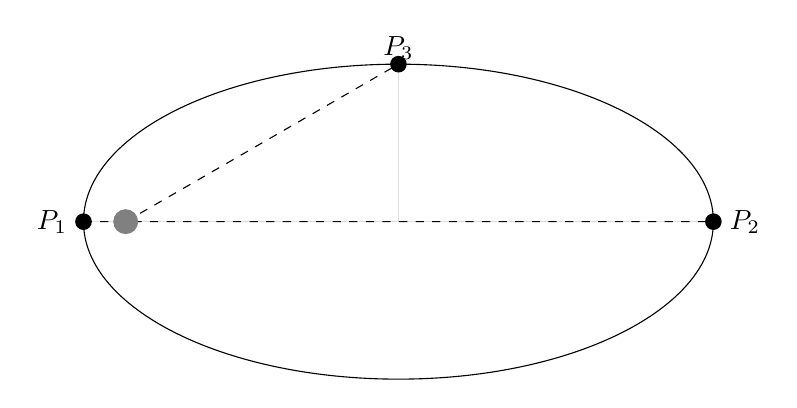
\begin{tikzpicture}
		% coordinates
		\coordinate (P1) at (-4,0);
		\coordinate (P2) at  (4,0);
		\coordinate (P3) at  (0,2);
		\coordinate (F)  at ({-sqrt(12)},0); % focus
		% ellipse
		\draw (0,0) ellipse (4cm and 2cm);
		% points
		\foreach\i in {1,2,3}
		\path[fill] (0,0) -- (P\i) circle (3pt) node[pos=1.1] {$P_\i$};
		% dashed lines
		\draw[dashed] (P1) -- (P2) (F) -- (P3);
		% focus
		\fill[gray] (F) circle (4.5pt);
	\end{tikzpicture}
\end{center}
The \textit{vis-viva equation} gives the orbital speed of an object travelling along the ellipse:
\begin{center}
$$v(x)=\sqrt {\mu \left(\frac {2} {x}- \frac {1} {a}\right),} \hspace{0.3in}\mu=G({m}_{1}+{m}_{2})$$
\end{center}
Here, $a$ is the semi-major axis, ${m}_{1}$ and ${m}_{2}$ are the masses of the orbiting bodies, $x$ is the distance between the comet and the centre of mass, and $G$ is the gravitational constant.\\
\textit{Answer:}\\
(a) Calculate the eccentricity of P/2023 IAAC's orbit around the Sun.\
\begin{itemize}
	\item Semi-major axis (a) = 16,5 AU
	\item Semi-minor axis (b) = 8,3 AU
\end{itemize}
We can use this formula to calculate the eccentricity:\\
$$e = \sqrt{1-\left(\frac {b}{a}\right)^{2}} = \sqrt{1-\left(\frac {8,3}{16,5}\right)^{2}}= 0,864 \hspace{0.1in}(high \hspace{0.08in}eccentricity)$$\\\
(b) Which one of the points ${P}_{1}$,${P}_{2}$,${P}_{3}$ is the aphelion and which one the perihelion?\
\begin{itemize}
	\item Perihelion is the point on a planet's orbit that is closest to the Sun. It is on the major axis. Then, aphelion is the point on a planet's orbit that is farthest from the Sun. It is on the major axis directly opposite the perihelion point. From this, we can conclude that perihelion represents on the point ${P}_{1}$ and the aphelion represents on the point ${P}_{2}$.
\end{itemize}
(c) Determine the comet's speed at three points ${P}_{1}$,${P}_{2}$,${P}_{3}$.
\begin{center}
	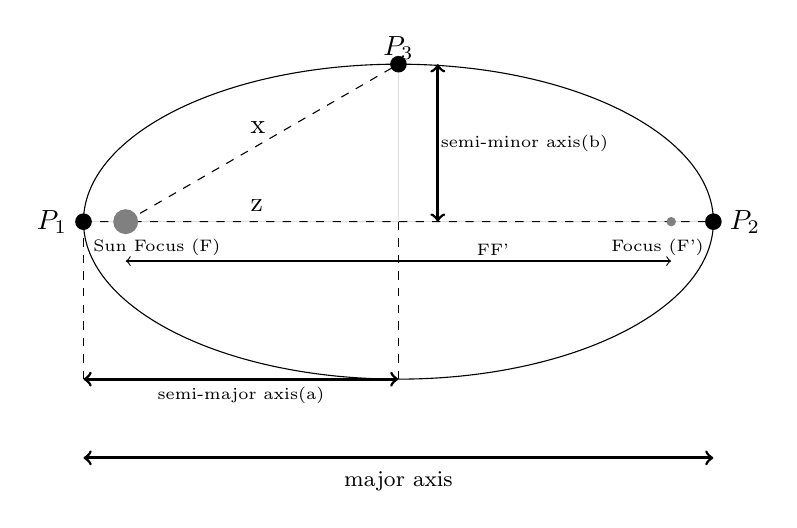
\begin{tikzpicture}
		% coordinates
		\coordinate (P1) at (-4,0);
		\coordinate (P2) at  (4,0);
		\coordinate (P3) at  (0,2);
		\coordinate (F1)  at ({-sqrt(12)},0); % focus
		\coordinate (F2)  at ({sqrt(12)},0); % focus
		% ellipse
		\draw (0,0) ellipse (4cm and 2cm);
		% points
		\foreach\i in {1,2,3}
		\path[fill] (0,0) -- (P\i) circle (3pt) node[pos=1.1] {$P_\i$};
		% dashed lines
		\draw[dashed] (P1) -- (P2) (F1) -- (P3);
		% focus
		\fill[gray] (F1) circle (4.5pt);
		\fill[gray] (F2) circle (1.7pt);
		% draw the vertical lines
		\draw[line width=1pt,<->] (0.5,0) -- (0.5,2) node[font=\fontsize{6}{10}\selectfont] at(1.6,1) {semi-minor axis(b)};
		\draw[dashed](-4,-0) -- (-4,-2);
		\draw[dashed](0,0) -- (0,-2);
		% draw the horizontal line
		\draw[<->] ({-sqrt(12)},-0.5) -- ({sqrt(12)},-0.5) node[font=\fontsize{6}{10}\selectfont] at (1.2,-0.36) {FF'};
		\draw[line width=1pt, <->](-4,-2) -- (0,-2) node[font=\fontsize{6}{10}\selectfont] at (-2,-2.2) {semi-major axis(a)};
		\draw[line width=1pt, <->] (-4,-3) -- (4,-3) node[font=\fontsize{8}{10}\selectfont] at (0,-3.3) {major axis};
		% add node
		\node [anchor=north west] at (-2,1.4) {x};
		\node [anchor=west] at (-2,0.2) {z};
		\node[font=\fontsize{6}{10}\selectfont,anchor=west] at (-4,-0.32) {Sun Focus (F)};
		\node[font=\fontsize{6}{10}\selectfont,anchor=east] at (4,-0.32) {Focus (F')};
	\end{tikzpicture}
\end{center}
\textit{Answer:}\\
First of all, calculate the ${r}_{a}$ and ${r}_{p}$. We know that $e=0,864$, we get
\begin{itemize}
	\item ${r}_{a} = (1+e)a = (1+0,864)16,5 = 30,69$ AU
	\item ${r}_{p} = (1-e)a = (1-0,864)16,5 = 2,31$ AU
\end{itemize}
Then, we get the major axis = ${r}_{a}+{r}_{p}= 33$ AU\\
Hence, we can determine the value of FF' = aphelion - perihelion = $(30,69-2,31)$AU = $28,38$ AU\\
To determine the value between the Sun and ${P}_{3}$, we can use the simple Pythagorean formula as follows:\\
Simply, we know that $ z = \left(\frac{1}{2}\right)FF' = 14,19$\hspace{0.1in}AU, so we can get the value of $x$\\
$x = \sqrt{(14,19)^{2}+(8,3)^{2}} = 16,44$ AU\\
Before we calculate the speed of each point, we can determine the value of $\mu$ (as we know the comet's mass negligible, the value of ${m}_{2}$ is 0)\\
$\mu =G({m}_{1}+{m}_{2})$\\
$\mu =G(M_{\odot})$\\
$\mu = 6,67 \times 10^{-11}$ m$^{3}$/kgs$^{2}$ $\cdot 1,9 \times 10^{30}$kg \\
$\mu = 1,267 \times 10^{20}$ m$^{3}$/s$^{2}$ \\ 
Finally, we can calculate the speed of each point as follows:\\
${r}_{a} = 30,69$ AU = $4,59 \times {10}^{12}$ m (${P}_{2}$)\\
${r}_{p} = 2,31$ AU = $3,46 \times {10}^{11}$ m (${P}_{1}$)\\
${r}_{x} = 16,44$ AU = $2,46 \times {10}^{12}$ m (${P}_{3}$)\\
$a = 16,5$ AU = $2,47 \times {10}^{12}$ m\\
$$v({r}_{a})=\sqrt {1,267 \times 10^{20} \left(\frac {2} {4,59 \times {10}^{12}}- \frac {1} {2,47 \times {10}^{12}}\right)} =1,98\times 10^{3} m/s $$\\
$$v({r}_{p})=\sqrt {1,267 \times 10^{20} \left(\frac {2} {3,46 \times {10}^{11}}- \frac {1} {2,47 \times {10}^{12}}\right)} =2,61\times 10^{4} m/s $$\\
$$v({r}_{x})=\sqrt {1,267 \times 10^{20} \left(\frac {2} {2,46 \times {10}^{12}}- \frac {1} {2,47 \times {10}^{12}}\right)} =7,21\times 10^{3} m/s $$\\\\
From the calculation above, we can conclude that the speed of comet P/2023 is greater at the perihelion point,${P}_{1}$, then comet's speed reach the smaller at the aphelion point, ${P}_{2}$.This is accordance to the Kepler's Second Law. At the perihelion point, the planet is at the closest distance to the Sun and is exposed stronger gravitational force, so the planet have a fastest speed to stay at the orbit. While the aphelion point, the planet is at the farthest distance from the Sun, so the gravitational force received by the planet slowest, the speed is also slowest, ${v}_{ra}<{v}_{rx}<{v}_{rp}$.


\paragraph{(Problem D: Distance Between Stars: 5 Points).}
Determining the distance to stars can be challenging. The parallax method is one way of finding the distance to many stars around us. Your research team measures the parallax of two stars that have a distance of 5 degrees from each other in the night sky: The first star has a parallax of 0,11 arcsec, and the second has a parallax of 0,13 arcsec. How far apart are the two stars from each other? Express your answer in light-years.\\
\textit{Answer:}\\
- From the small angle equation, we have
$$ p = 206.265 \cdot \frac{D}{d}$$
-Where the Earth-Sun distance (1 AU), d is the distance to the star, and p is the parallax angle in arcseconds($"$). One \textbf{parsec} (pc) is 206.265 AU, and the distance in parsecs is given by
$$d (pc) = \frac{1}{p(")}$$\\
-From the formula above, we can measure the distance of the first and second star as ${d}_{1}$ and ${d}_{2}$,
\begin{itemize}
	\item ${d}_{1} = \frac{1}{{p}_{1}} = \frac{1}{0,11} = 9,09$ parsecs
	\item ${d}_{2} = \frac{1}{{p}_{2}} = \frac{1}{0,13} = 7,69$ parsecs
\end{itemize}
-After we know the distance of each stars and the angle ($\theta$ = 5 degrees = 0,087 rad), now we can calculate the distance between stars using Trigonometry rules as follows:
\begin{center}
$d=\sqrt{({d}_{1})^{2}+({d}_{2})^{2}-2{d}_{1}{d}_{2}cos\theta}$
$$d= \sqrt{(9,09)^{2}+(7,69)^{2}-2(9,09)(7,69)cos(0,087)}$$
$$d= \sqrt{(82,63)+(59,14)-(139,80)(0,9)}$$
$$d= \sqrt{(141,77-125,82)}$$
$d$ = 3,99 parsecs or 13,01 light-years\\
\end{center}


\paragraph{Problem E: Dark Energy (5 Points).}
Cosmology studies the dynamics of the universe on its largest scales. Its research reveals how the universe evolves over time and, in particular, how it expands. The term \textit{dark energy} frequently appears in cosmology. What does the term dark \textit{dark energy} describe? What are evidences for the existence of dark energy?\\
\textit{Answer:}

There are two dominant compositions that fill the universe: dark matter and dark energy. The two compositions are still a mystery because astronomers are still unsure of their physical properties and we also cannot see dark matter and dark energy. One of these is dark energy, which is believed to be the cause of the expansion of the universe. To date, there is no direct evidence that dark energy exist. However, there are some phenomena in the universe that indicate the existence of dark energy, such as the observed acceleration of the expansion of the universe. In addition, gravitational lensing obervations and cosmological calculations suggest that more matter must exist in the universe than we directly observe, and dark energy is the puzzle that explains the missing piece. However, the explanation of dark energy is still a matter of scientific research and debate.\

The first foray into exploring the mystery of dark energy began in 1929, when astronomer Edwin Hubble found evidence that the universe was expanding. Hubble's observations showed that galaxies outside the solar system were moving away from Earth at an increasing speed with increasing distance. This discovery was made by observing Type Ia Supernovae far beyond our galaxy. Using this galaxy as "standard candles" astronomers were able to measure the distance of cosmic objects across the universe.\

Then in 1988, astronomers found more evidence that the expansion of the universe was not in line with general relativity. In this discovery, astronomers named the mysterious energy riving the expansion as dark energy. All of this observational evidence suggest that dark energy plays an important role shaping the structure of the universe as we see today.












\end{document}
